\documentclass[11pt]{article}
\usepackage{amsmath}
\usepackage{geometry}                % See geometry.pdf to learn the layout options. There are lots.
\geometry{letterpaper}                   % ... or a4paper or a5paper or ... 
%\geometry{landscape}                % Activate for for rotated page geometry
%\usepackage[parfill]{parskip}    % Activate to begin paragraphs with an empty line rather than an indent
\usepackage{graphicx}
\usepackage{amssymb}
\usepackage{epstopdf}
\DeclareGraphicsRule{.tif}{png}{.png}{`convert #1 `dirname #1`/`basename #1 .tif`.png}

%Don't list section numbers
\setcounter{secnumdepth}{0}

\title{CS 1653: Applied Cryptography and Network Security\\Term Project, Phase 4}
\author{Lindsey ``Hellman" Bieda\quad\texttt{leb35@pitt.edu}\\Tucker ``Diffie" Trainor\quad\texttt{tmt33@pitt.edu}}
\date{April 5, 2012} % Activate to display a given date or no date

\begin{document}
\maketitle
\section{Introduction: Cryptographic Techniques}
The additional threats to our Secure File Server model present new challenges to ensuring the confidentiality and integrity of a user's data. To protect against these threats, we can introduce cryptographic techniques that either augment or supplement existing methods that addressed Threats 1-4.

We will continue to use AES for symmetric key encryption, and to ensure against tampering of AES encrypted messages we will employ HMAC with SHA1 to authenticate messages sent over an encrypted channel. Embedding sequence numbers into messages will also help in detecting replay or reordering by a malicious agent. To combat against file leakage and maintain group privileges over file access, files saved on any File Server will be encrypted with AES, the keys of which will be maintained by the Group Server, which will generate keys by leveraging a combination of an asymmetric key encryption and a hash function against unique properties of a file and group version control. 
% Threat 5
\section{Threat 5: Message Reorder, Replay, or Modification}
\subsection{Threat Description}
Whereas Threats 1-4 encompassed the possible efforts of a \emph{passive} attacker that could only eavesdrop on connections between clients and servers, Threat 5 now introduces the danger of an \emph{active} attacker who is capable of inserting, reordering, replaying, or modifying messages. Though encryption of the communication channel was enough to thwart a passive attacker and maintain confidentiality, an active attacker is able to disrupt the integrity of communications by effectively nullifying messages by tampering with them.

Reordering and replaying of messages can convince either end of a communication channel that the other party wishes to perform an action that is not what is actually intended by that party despite the correctness of the mechanism. An active attacker can also alter the message itself at the bit level, causing changes that could randomly alter the intention of the message or garble it completely. Modification is not only an affront to the integrity of the Secure File Server model but also can reduce availability if no message can be trusted as to its accuracy.
\subsection{Mechanism Description}
The mechanism builds upon the protocols used in Threats 1-4 that establish a secure session key between a client and a server. Though messages passed in the session are secure from eavesdropping, they are not secure from reorder, replay, or modification. We use two methods to eliminate these new threats: sequence numbers and message authentication.

Sequence numbers are a simple yet effective tool that would alert either end of channel that a message has ben reordered or replayed. We modify our message format so that it includes an integer field to store the sequence number. Then, after receiving a message, the receiving party increments the sequence number by 1 and uses that value in their response. Replays and reordering of messages are easily detectable by either party, as the sequence number will reveal an inconsistency.

Message authentication is a cryptographic principal that is used to verify that a message has not been tampered with. We have chosen the HMAC with SHA1 protocol to authenticate messages. To use HMAC in the most secure manner, we need to create an additional shared secret key to use for the keyed hash of HMAC. We can do this at the same time as the creation of the shared secret key for the AES symmetric encryption. With these two keys, k$_\text{e}$ for encryption and k$_\text{a}$ for authentication, we can create an authentication mechanism that addresses Threat 5. The sequence number and message are encrypted with k$_\text{e}$, and then the HMAC is done using k$_\text{a}$ on the encrypted sequence number and message (see Figure \ref{threat5}). The receiver of the encrypted message and HMAC digest will then be able to verify against tampering.
\begin{figure}[htbp]
\begin{center}
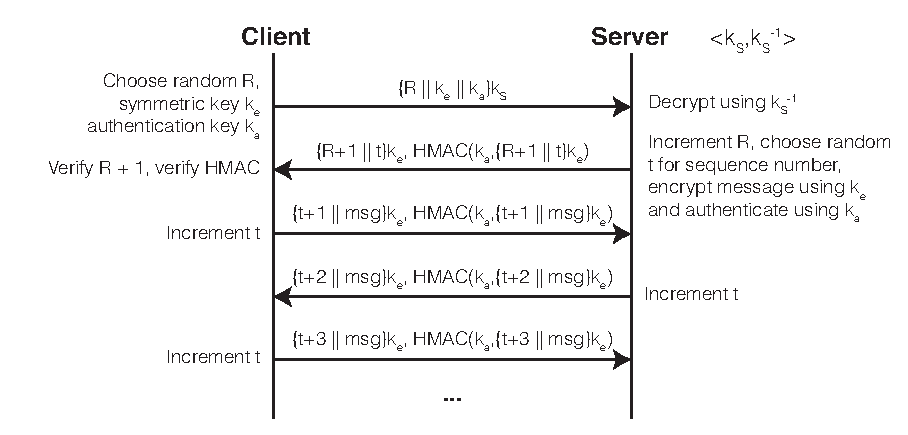
\includegraphics{threat5.eps}
\caption{Threat 5 Mechanism}
\label{threat5}
\end{center}
\end{figure}
\subsection{Correctness and Security of Mechanism}
%%%%%%%%%% NEED TO COMPLETE
Lastly, provide a short argument addressing why your proposed mechanism sufficiently addresses this particular threat. This argument should address the correctness of your approach, as well as its overall security. For example, if your mechanism involves a key agreement or key exchange protocol, you should argue that both parties agree on the same key (correctness) and that no other party can figure out the key (security).
% Threat 6
\section{Threat 6: File Leakage}
\subsection{Threat Description}
The threat of file leakage represents a major vulnerability of the previous set of threats to our model. Previously, files saved to a File Server were encrypted over the network but not in storage. Therefore, an untrusted File Server could leak fully readable files that any user, malicious or not, could read. Obviously, we must encrypt the files to protect them against unauthorized access, but at the same time we must also enforce group privileges where group members have access to the files and security from former group members is maintained.
\subsection{Mechanism Description}
If groups were limited to just their owners, the threat could easily be eliminated with a single secret key for all files that was only known by or accessible to the owner. However, the fluid nature of groups quickly complicates this ideal and requires a more elaborate mechanism.

We start with a master version integer V$_\text{M}$, which represents the current iteration of a group. The value of V$_\text{M}$ is kept in a hash table (see Figure \ref{threat6}) on the Group Server and its key is the name of the group. As new or modified files are uploaded to a File Server, they are assigned a version number V which is equal to whatever V$_\text{M}$ is at the time of upload. The unique properties of the file (e.g. its group, owner, and file path) are used as the key in the hash table to place the value of V. Whenever a file needs to be downloaded, its unique properties are used to retrieve the file's version number, which in turn is used to generate its secret symmetric key for encryption and decryption.
\begin{figure}[htbp]
\begin{center}
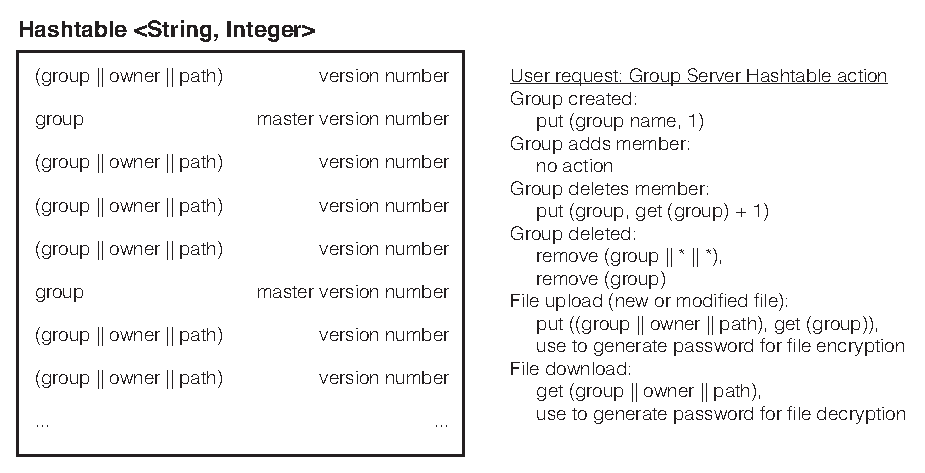
\includegraphics{threat6.eps}
\caption{Threat 6 Mechanism: Hashtable and Operations}
\label{threat6}
\end{center}
\end{figure}
The Group Server handles the creation of the symmetric key as well. When the key is needed, the Group Server creates an array of bytes consisting of the unique file properties, concatenates the version number of the file onto that array (either V$_\text{M}$ for a new or modified file, V for an existing file), and then encrypts that array with its private key k$_\text{G}^{-1}$ using RSA. To prevent possible excessive exposure of private key encryptions, the encrypted data is then subjected to a 256-bit SHA hash to provide the final key that will be used for final encryption. The use of 256-bit SHA instead of the 160-bit SHA1 hash is twofold: the extra bits provide increased confidentiality and a 256-bit value is easily usable for 256-bit AES encryption.

Once the key is created, the Group Server can send it over a secure channel to the Client, whose software need not expose it to him/her but simply use it to encrypt the data that is being sent to the File Server (see Figure \ref{threat6a}) or decrypt data being received from the File Server (see Figure \ref{threat6c}). Thus, the Client and Group Server are the only parties who have any access to the key, leaving a malicious or leaky File Server with encrypted files that are of little use to anyone but authenticated group members.
\begin{figure}[htbp]
\begin{center}
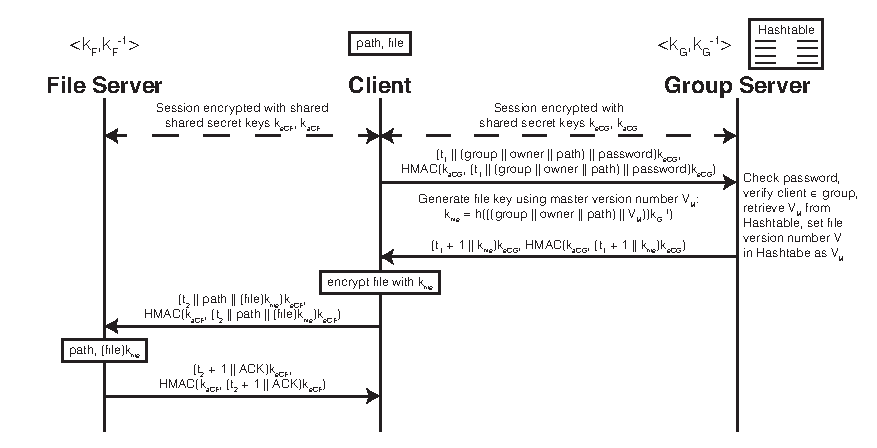
\includegraphics{threat6a.eps}
\caption{Threat 6 Mechanism: Upload Diagram}
\label{threat6a}
\end{center}
\end{figure}
\begin{figure}[htbp]
\begin{center}
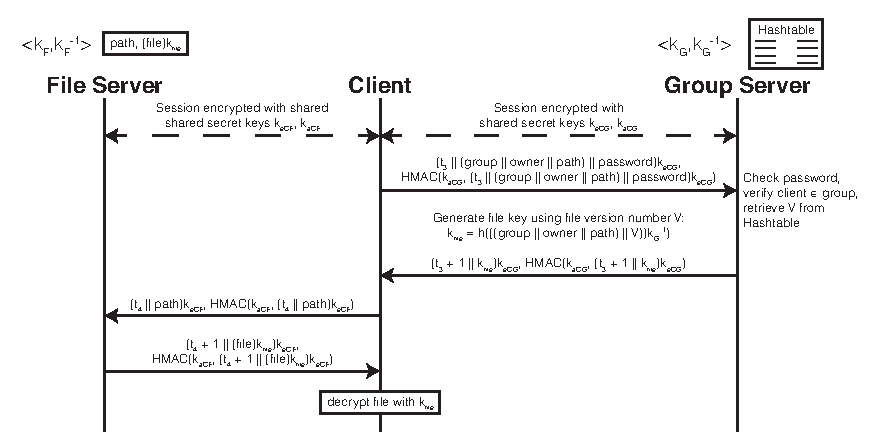
\includegraphics{threat6c.eps}
\caption{Threat 6 Mechanism: Download Diagram}
\label{threat6c}
\end{center}
\end{figure}
\subsection{Correctness and Security of Mechanism}
To illustrate the security of the mechanism, we need to fully explain the handling of version numbers and how it affects forward and backward secrecy as group membership changes. As shown in Figure \ref{threat6}, the typical event that changes the master version number V$_\text{M}$ is when a member is removed from a group.
% Threat 7
\section{Threat 7: Token Theft}
\subsection{Threat Description}
stub
\subsection{Mechanism Description}
(see Figure \ref{threat7})
\begin{figure}[htbp]
\begin{center}
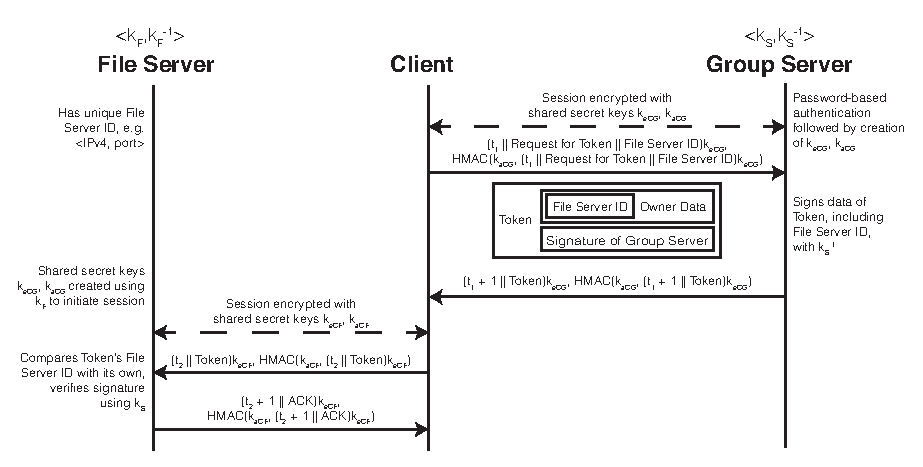
\includegraphics{threat7.eps}
\caption{Threat 7 Mechanism}
\label{threat7}
\end{center}
\end{figure}
\subsection{Correctness and Security of Mechanism}
stub
\section{Discussion and Commentary}
After completing one section for each threat, conclude with a paragraph or two discussing the interplay between your proposed mechanisms, and commenting on the design process that your group followed. Did you discuss other ideas that didn�t pan out before settling on the above-documented approach? Did you end up designing a really interesting protocol suite that addresses multiple threats at once? Use this space to show off your hard work!
\section{Threats 1 through 4 revisited}
Finally, spend about one paragraph convincing me that your modified protocols still address the threats T1-T4 described in Phase 3 of the project. Full credit for Phase 4 requires that all Phase 3 threats are still protected against.
\end{document}
